\documentclass[a4paper,11pt]{report}
\usepackage[T1]{fontenc}
\usepackage[utf8]{inputenc}
\usepackage{lmodern}
\usepackage{graphicx}

\title{\textbf{Sprawozdanie z laboratorium\\tablica asocjacyjna}}
\author{Adam Dąbrowski 184208}
\begin{document}
\maketitle
\chapter{Wprowadzenie}

Celem ćwiczenia było zapoznanie się z tablicą asocjacyjną w tym tablicą haszującą. 

\chapter{Realizacjia}
  
\newpage 
\section{Tablica asocjacyjna}

Złożoność obliczeniowa \\
dodawanie elemntu - $O(1)$\\  
usuwanie  element - $O(n)$\\
wyszukiwanie elementu- $O(n)$\\
\begin{tabular}{|rl|}
\hline
\multicolumn{2}{|c|}{wczytywanie danych}\\
\hline
ilosc elementow & czas [$\mu s$]\\
\hline
1&8\\
10&14\\
100&38\\
1000&309\\
10000&3428\\
100000&34624\\
\hline
\end{tabular}
\\
\begin{tabular}{|rl|}
\hline
\multicolumn{2}{|c|}{wyszukiwanie}\\
\hline
ilosc elementow & czas [$\mu s$]\\
\hline
1&5\\
10&8\\
100&223\\
1000&19371\\
10000&1961250\\
\hline
\end{tabular}
\\
\includegraphics[angle=270, scale = 0.5]{wykresy/wczytywanie.eps}
\includegraphics[angle=270, scale = 0.5]{wykresy/wyszukiwanie.eps}
\newpage
\section{tablica haszująca}
Złożoność obliczeniowa\\ 
dodawanie elemntu - $O(1)$\\  
usuwanie  element - $O(1)$\\
wyszukiwanie elementu- $O(1)$\\
  
\begin{tabular}{|rl|}
\hline
\multicolumn{2}{|c|}{wczytywanie danych}\\
\hline
ilosc elementow & czas [$\mu s$]\\
\hline
1&8\\
10&18\\
100&111\\
1000&1235\\
10000&13350\\
100000&158881\\
\hline
\end{tabular}
\newline
\newline
\begin{tabular}{|rl|}
\hline
\multicolumn{2}{|c|}{wyszukiwanie}\\
\hline
ilosc elementow & czas [$\mu s$]\\
\hline
1&15\\
10&23\\
100&206\\
1000&2308\\
10000&26129\\
100000&380506\\
\hline
\end{tabular}
\\
\includegraphics[angle=270, scale = 0.5]{wykresy/wczytywanie_hash.eps}
\includegraphics[angle=270, scale = 0.5]{wykresy/wyszukiwanie_hash.eps}

\chapter{Wnioski}
Czasy wczytywania w obu tablicach były zbliżone, jednak w tablicy haszującej nieco większe. Dzieje się tak, ponieważ wyliczanie indeksu tablicy w funkcji haszującej zajmuje dodatkowy czas, ponadto zaimplementowałem ją jako vector, a tablicę bez haszowania jako listę co też ma wpływ na różnice w czasie wczytywania. Podczas wyszukiwania pobierałem z tablicy wszysktie elementy jakie do niej wczytałem. W tablicy asocjacyjnej bez haszowania wyszukiwanie zależy bezpośrednio od wielkosci pojemnika w najgorszym wypadku musimy przejść przez wszystkie elementy zanim znajdziemy ten, którego szukamy. W tablicy haszującej czas wyszukiwania zalezy od tego jak dobrze uda nam się dopasować funkcję haszującą do danych wejściowych - w najgorszym wypadku tworzy nam się lista o długości n w pierwszej komórce tablicy jednak zakładamy, że dobrze dobralismy funkcje haszujaca i taka sytuacja nigdy nie zachodzi. Wtedy czas wyszukiwania jest bliski $O(1)$ ponieważ musimy użyć funkcji haszującej do wyliczenia indeksu danego elementu tablicy, a następnie przejżeć listę elementów w tej komórce. W moim przypadku dla 10000 elemntów najdłuższa napotkana lista miała 9 elementów. Jeżeli wiemy jakich danych wejściowych możemy się spodziewać tablica haszująca jest bardzo dobrym rozwiązaniem. Pod spodem wstawiam wykres, na którym porównuję czasy wyszukiwania dla wyżej wymienionych tablic.
\includegraphics[angle=270, scale = 0.5]{wykresy/wyszukiwanie_porownanie.eps}
\end{document}
